% !TeX program = pdflatex
\documentclass[border=6pt]{standalone}
\usepackage{tikz}
\usetikzlibrary{arrows.meta, positioning, calc, decorations.pathreplacing}

\definecolor{MediumRed}{rgb}{0.925, 0.345, 0.345}
\definecolor{MediumGreen}{rgb}{0.37, 0.7, 0.66}
\definecolor{MediumBlue}{rgb}{0.015, 0.315, 0.45}
\definecolor{DarkBlue}{rgb}{0.05, 0.15, 0.35}

% y = BLEU-4 * 0.26 cm
\begin{document}
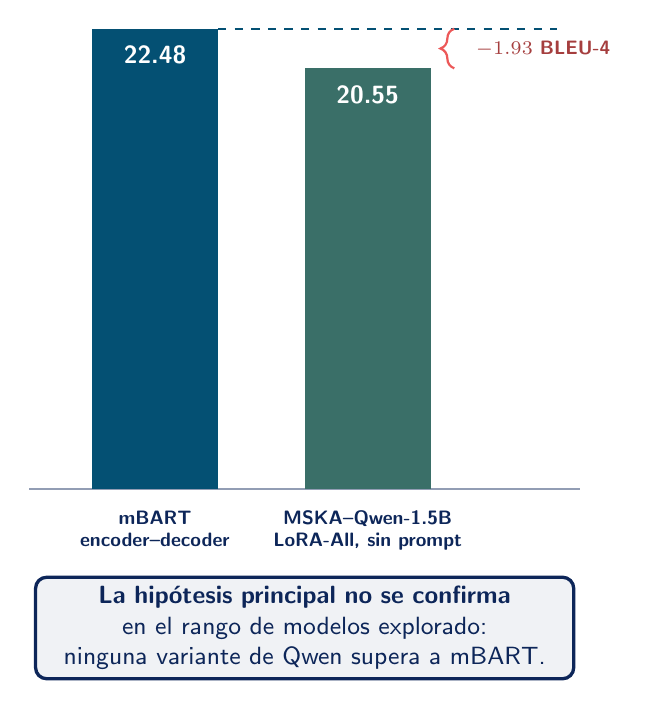
\begin{tikzpicture}[font=\sffamily]

% eje base
\draw[DarkBlue!45, line width=1pt] (-0.3,0) -- (6.7,0);

% --- barra mBART (referencia) ---
\fill[MediumBlue] (0.5,0) rectangle (2.1,{22.48*0.26});
\node[font=\sffamily\small\bfseries, text=white, anchor=north] at (1.3,{22.48*0.26-0.1}) {22.48};
\node[font=\sffamily\scriptsize\bfseries, text=DarkBlue, anchor=north, align=center] at (1.3,-0.15)
    {mBART\\\scriptsize\textit{encoder--decoder}};

% --- barra mejor Qwen ---
\fill[MediumGreen!62!black] (3.2,0) rectangle (4.8,{20.55*0.26});
\node[font=\sffamily\small\bfseries, text=white, anchor=north] at (4.0,{20.55*0.26-0.1}) {20.55};
\node[font=\sffamily\scriptsize\bfseries, text=DarkBlue, anchor=north, align=center] at (4.0,-0.15)
    {MSKA--Qwen-1.5B\\\scriptsize LoRA-All, sin \textit{prompt}};

% --- linea de referencia mBART ---
\draw[MediumBlue, dashed, thick] (2.1,{22.48*0.26}) -- (6.4,{22.48*0.26});

% --- brecha ---
\draw[decorate, decoration={brace, amplitude=5pt}, MediumRed, thick]
    (5.1,{20.55*0.26}) -- (5.1,{22.48*0.26});
\node[font=\sffamily\scriptsize\bfseries, text=MediumRed!70!black, anchor=west] at (5.25,{21.5*0.26})
    {$-1.93$ BLEU-4};

% --- veredicto ---
\node[draw=DarkBlue, very thick, rounded corners=4pt, fill=DarkBlue!6, text=DarkBlue,
      align=center, font=\sffamily\small, text width=6.6cm, anchor=north] at (3.2,-1.1)
    {\textbf{La hipótesis principal no se confirma} en el rango de modelos explorado:\\
     ninguna variante de Qwen supera a mBART.};

\end{tikzpicture}
\end{document}
